\documentclass[a4paper]{ltjsarticle}

\usepackage[dvipdfmx]{graphicx}
\usepackage[dvipdfmx,hidelinks,pdfusetitle]{hyperref}
\hypersetup{
    colorlinks=false,
    bookmarksnumbered=true,
    pdfborder={0 0 0},
    bookmarkstype=toc
}
\usepackage[nobreak]{cite}
\usepackage{pxjahyper}
\usepackage{amsmath}
\usepackage{tikz}

\usetikzlibrary{datavisualization}
\usetikzlibrary{positioning}
\usetikzlibrary{shapes.geometric, shapes.misc}
\usetikzlibrary{patterns}
\usetikzlibrary{calc}

\begin{document}

\begin{itembox}[l]{東京大学 2013年 文科 第2問}
    座標平面上の3点

    \begin{equation*}
        P(0,\ -\sqrt{2}),\ Q(0,\ \sqrt{2}),\ A(a,\ \sqrt{a^2+1})\quad (0\leq a\leq 1)
    \end{equation*}

    を考える.

    \begin{enumerate}[label=(\arabic*)]
        \item 2つの線分の長さの差 $\mathrm{PA}-\mathrm{AQ}$ は $a$ によらない定数であることを示し,その値を求めよ.
        \item Q を端点とし A を通る半直線と放物線 $y=\frac{\sqrt{2}}{8}x^2$ との交点を B とする.点 B から直線 $y=2$ へ下ろした垂線と直線 $y=2$ との交点を C とする.このとき,線分の長さの和

              \begin{equation*}
                  \mathrm{PA}+\mathrm{AB}+\mathrm{BC}
              \end{equation*}

              は $a$ によらない定数であることを示し,その値を求めよ.
    \end{enumerate}
\end{itembox}

\begin{enumerate}[label=(\arabic*)]
    \item

          \begin{figure}[!ht]
              \centering
              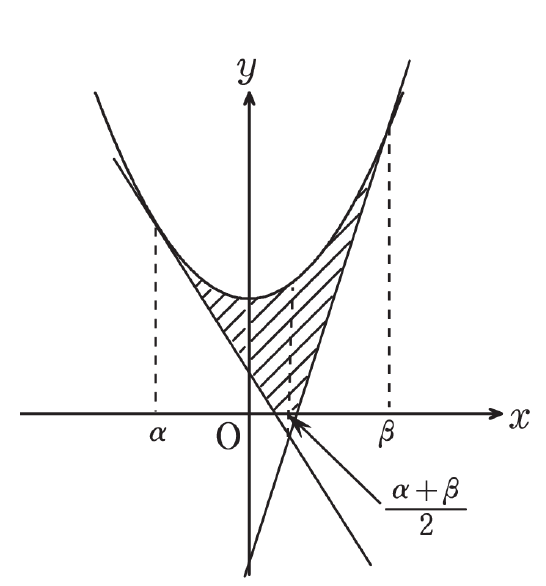
\includegraphics[width=0.5\textwidth]{f1.png}
          \end{figure}

          \begin{align*}
              \mathrm{PA} & =\sqrt{a^2+(\sqrt{a^2+1}+\sqrt{2})^2} \\
                          & =\sqrt{2a^2+3+2\sqrt{2a^2+2}+1}       \\
                          & =\sqrt{(\sqrt{2a^2+2}+1)^2}           \\
                          & =\sqrt{2a^2+2}+1                      \\
          \end{align*}

          同様に,

          \begin{align*}
              \mathrm{AQ} & =\sqrt{a^2+(\sqrt{a^2+1}-\sqrt{2})^2} \\
                          & =\sqrt{2a^2+2}-1
          \end{align*}

          よって,

          \begin{equation*}
              \mathrm{PA}-\mathrm{AQ}=\sqrt{2a^2+2}+1-(\sqrt{2a^2+2}-1)=2
          \end{equation*}

    \item Q, A, B は一直線上にあるため (1) の結果を用いて,

          \begin{equation}
              \mathrm{PA}+\mathrm{AB}+\mathrm{BC}=2+\mathrm{AQ}+\mathrm{AB}+\mathrm{BC}=2+\mathrm{QB}+\mathrm{BC}\label{eq:1}
          \end{equation}

          半直線 AQ:$y=\frac{\sqrt{a^2+1}-\sqrt{2}}{a}x+\sqrt{2}\ (x\geq 0)$ と放物線 $y=\frac{\sqrt{2}}{8}x^2$ の交点を B$(x_B,\frac{\sqrt{2}}{8}{x_B}^2)$ とおく.図より, A は $y\leq \sqrt{2}$ にあり, B は $x\geq 0, y<2$ にあって,

          \begin{align*}
              \mathrm{QB} & =\sqrt{{x_B}^2+\left(\frac{\sqrt{2}}{8}{x_B}^2-\sqrt{2}\right)^2} \\
                          & =\sqrt{\left(\frac{\sqrt{2}}{8}{x_B}^2+\sqrt{2}\right)^2}         \\
                          & =\frac{\sqrt{2}}{8}{x_B}^2+\sqrt{2}                               \\
              \mathrm{BC} & =2-\frac{\sqrt{2}}{8}{x_B}^2
          \end{align*}

          よって,\eqref{eq:1} より,

          \begin{align*}
              \mathrm{PA}+\mathrm{AB}+\mathrm{BC} & =2+\frac{\sqrt{2}}{8}{x_B}^2+\sqrt{2}+2-\frac{\sqrt{2}}{8}{x_B}^2 \\
                                                  & =4+\sqrt{2}
          \end{align*}
\end{enumerate}



\end{document}
